\chapter{Cottontail DB}
\label{chapter:cottontaildb}

\emph{Cottontail DB}~\cite{Gasser:2020cottontail} is our reference implementation for the query, cost and index-models described in \Cref{chapter:system_model}. Starting out as a drop-in replacement for ADAMpro \cite{Giangreco:2016adam}, it has grown to be a full fledged \acrshort{dbms} with support for classical boolean retrieval as well as proximity based search. Both aspects have been combined in a unified query and execution model and many explicit and implicit design decisions went into the system, which are outlined in this chapter.

\emph{Cottontail DB} is written in Kotlin\footnote{See: https://kotlinlang.org/} and runs on the \acrfull{jvm}. While an unorthodox choice of language and environment for a database, there are several prominent examples that were built for the \acrshort{jvm}, including but not limited to H2\footnote{See: http://hsqldb.org/}, HSQLDB\footnote{See: http://hsqldb.org/} or Derby\footnote{See: https://db.apache.org/derby/}. \emph{Cottontail DB}'s source code can be downloaded from GitHub\footnote{See: https://github.com/vitrivr/cottontaildb}. It is freely available under a permissive open source license and can be used as standalone application, Docker container or in an embedded mode.

\section{Architecture}

The main components of the \emph{Cottontail DB} stack are depicted in \Cref{figure:cottontail_architecture}. We use the path of a query, indicated by the red and green arrows, to illustrate the components involved in query execution.

At a high level, every query must undergo \emph{parsing}, \emph{binding}, \emph{planning} and \emph{execution}. Access to the data is facilitated by a storage manager that delegates low level I/O to a storage engine. 

\begin{figure}[bt]
    \centering
    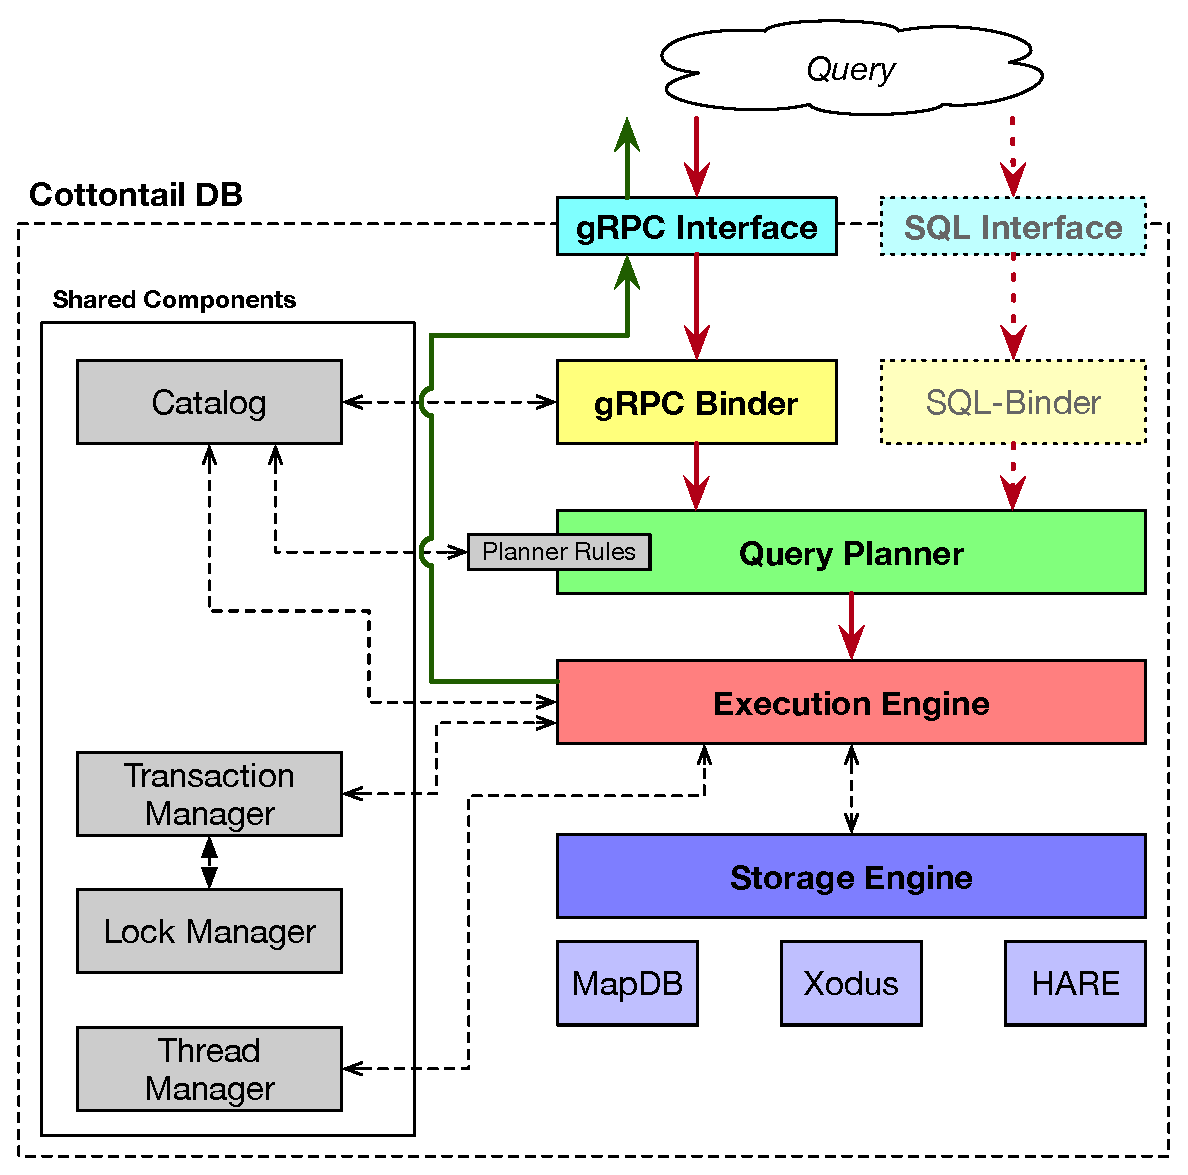
\includegraphics[width=\textwidth]{figures/architecture.eps}
    \caption{Architecture diagram depicting the main components of Cottontail DB. The coloured arrows indicate the path a query takes within the system. The dashed arrows indicate interactions between components.}
    \label{figure:cottontail_architecture}
\end{figure}

\subsection{Query Parsing and Binding}
As every \acrshort{dbms}, \emph{Cottontail DB} uses a query language that allows for interaction with other systems. These interactions include data definition, data management, transaction management and the formulation of queries. In its current version, \emph{Cottontail DB} uses a query language based on \emph{gRPC}\footnote{See: https://grpc.io/}, hence, all queries are expressed as \emph{Protocol Buffer}\footnote{See: https://developers.google.com/protocol-buffers/} messages. Internally, the gRPC endpoint is a collection of four services for handling \acrshort{ddl}, \acrshort{dml}, \acrshort{dql} and transaction management messages. The parsing of incoming messages, the mapping of messages to the correct service and endpoint and low-level handling of communication with clients is delegated to the gRPC Kotlin library. 

The reason for the choice of gRPC is threefold: Firstly, Cottontail DB's predecessor -- ADAMpro -- already used and introduced gRPC into the \emph{vitrivr} stack. Consequently, building on this work greatly simplified the task of integrating \emph{Cottontail DB}. Secondly, gRPC -- being a platform independent remote procedure call framework -- introduces out-of-the-box support for a large range of programming environments. As of now, there is a Java\footnote{See: https://github.com/vitrivr/cottontaildb-proto/} and a Python\footnote{See: https://github.com/Spiess/cottontaildb-python-client/} client for Cottontail DB. And finally, the gRPC Kotlin library greatly simplified the task of structuring query endpoints, parsing incoming query messages and handling the query responses.

Regardless of the use of gRPC, Cottontail DB is compatible with the SQL standard insofar as it supports a specific feature. This was shown by be the successful integration of \emph{Cottontail DB} as a storage engine for \emph{Polypheny DB} \todo{Ref: Polypheny DB + joint publication}. Consequently, it is possible to add additional endpoints that can accept, e.g., \acrshort{sql} queries. However, for complete SQL compliance, one would have to add some language features that are currently not supported by \emph{Cottontaild DB} (e.g., JOINS). Furthermore, handling the technical details of parsing the incoming query and communication with the client must be handled as well.

Irrespective of its source, any incoming query message undergoes a \emph{binding} step in \emph{Cottontail DB}. Query binding includes three important aspects:

\begin{enumerate}
    \item Names that reference database objects such as entities, columns and indexes are resolved using \emph{Cottontail DB}s catalogue and replaced by concrete instances of the respective object.
    \item Literal values, e.g., in predicates, are extracted and cached for late binding. This allows for reuse of execution plans with different values.
    \item The parsed message is converted into a \emph{canonical operator node tree} that logically represents the query.
\end{enumerate}

The result of the parsing and binding step is the canonical operator node tree as a logical and unoptimized query representation.  Every node in the tree represents and operator that acts on a single \emph{record} or \emph{tuple} and must be executed in order to generate the desired result. The conversion of a message to a tree is performed in a naive manner and only syntactic checks and optimization are performed at this stage (e.g., type checks, removal of trivial predicates such as ``$1 = 1$'').

\subsection{Query Planner}

The goal of the query planner is to find a cost-optimal execution plan for a query given the \emph{policy} valid for the current query context and \emph{Cottontail DB}'s cost model. The input into the query planner is the canonical operator node tree resulting from the binding stage.

Query planning in \emph{Cottontail DB} takes place in three steps: First, and optionally, the canonical operator node tree is compared to the \emph{plan cache}. If the cache contains a hit for that tree, the optimized plan in the cache can be re-used and all the subsequent steps can be skipped. Second, if there is no hit in the cache or the cache is bypassed, the canonical operator node tree undergoes \emph{optimization}. Optimization step generates different versions of the input plan by applying optimization rules that act on and manipulate the tree to generate new plans. Finally, once optimization has concluded, the  plan that minimizes the expected cost is selected and \emph{implemented}.

\subsubsection{Basic Optimization Algorithm}

The query planner used by \emph{Cottontail DB} is rather naive and can be categorized as a rule-based query planner. As the name implies, it generates new plans by enumerating and applying a set of rules to the input plan(s) in a recursive fashion. These rules recognize patterns in the structure of the \emph{operator node tree} and try to re-arange and/or replace nodes in the tree to generate a more optimal but equivalent version of the plan.

The optimization follows the same, basic algorithm: An input plan is enumerated and the planner tries to apply every rule in the ruleset to every node in the plan. If a rule can be applied to a node, the resulting, new query plan is stored in the memoization table along with the input plan for future reference. Every planning stage involves a defined number of passes, and the output of every pass acts as the input for the next. Consequently, all the intermediate plans generated by one pass are run through the same algorithm and allthe rules again for the next pass.

Since applying a rule to a may result in another tree plus the input tree, which in turn can again be optimized, the search space grows exponentially with the complexity of the input plan and the number of rules to apply. To address this, \emph{Cottontail DB}'s query planner employs certain heuristics to keep the search space manageable:

\begin{enumerate}
    \item Very large, complex plans (e.g., stemming from sub-selects or JOINs) are broken into groups and every group is optimized and treated as an isolated plan. The assumption being that the combination of smaller, near-optimal plans must be close to optimal as well.
    \item The planning of every group is done in two stages -- a \emph{logical} and \emph{physical} stage -- with distinct and disjoint sets of rules. The results of the logical stage act as an input for the physical stage.
    \item Logical and physical query plans are uniquely identified by a hash. Memoization in combination with the aforementioned hash is used to track trees that have already been optimized and skip them (dynamic programming).
    \item Physical execution plans are actively pruned by the planner between the different passes based on the cost estimate for the plan.
\end{enumerate}

Between the logical and the physical planning, there is an implementation step that maps every logical operator node to its naive, physical counterpart. The number of passes per stage and active pruning of plans during the physical phase are used to steer the high-level behaviour of the query planner. During the logical phase, the goal is to generate as many, equivalent, logical query representations as possible to have something to optimize (expansion phase). During the physical phase, the planner tries to limit the number of intermediate plans.

\subsubsection{Plan Caching}

The plan cache is an optimization mechanism that amortizes the cost of the expensive query planning if a certain type of query is executed multiple times. Basically, it assigns a unique hash code to every incoming \emph{canonical operator node tree} and maps the resulting, optimized physical plan to that hash in memory. If the same query is processed again, that plan can be re-used directly and another round of planning can be avoided.

While great in theory, there are certain limitations to the plan cache mechanism in \emph{Cottontail DB}, which is why it is currently disabled by default. Firstly, the actual execution performance of a plan in not being evaluated against the cost model, i.e., the level of optimality of an execution plan is not assessed. And secondly, there is no mechanism that invalidates entries as changes to the data occur. 

\subsubsection{Logical Optimization}
\subsubsection{Physical Optimization}


\subsection{Query Execution}


\subsection{Storage}
\subsubsection{MapDB}
\subsubsection{Xodus}
\subsubsection{HARE}



\section{Additional Functionality}

\todo[inline]{Implementation chapter for Cottontail DB}